% !TeX root = ../main.tex

\section{Clustering}

\paragraph{Variants of k-means:}
For clustering see section 14 of ``The Elements of Statistical Learning'' (Hastie, Tibshirani, Friedman - 2009). Section 14.3 ``Cluster Analysis'' introduces different flavours of k-means. Points of interest are:
\begin{itemize}
	\item Proximity Matrices
	\item K-means
	\item Gaussian Mixtures as Soft K-means Clustering
	\item Vector Quantization
\end{itemize}

\paragraph{Q:} How can we determine k?

Let $w(c)$ be distance from samples to cluster centers within clusters. We use this as a metric of quality in cluster analysis.

\subparagraph{Approach 1:} Track the rate of change of a quality metric (like $w(c)$). Proposed in ``Pattern Classification'' (Duda, Hart, Stork).

\begin{figure}[H]
	\centering
	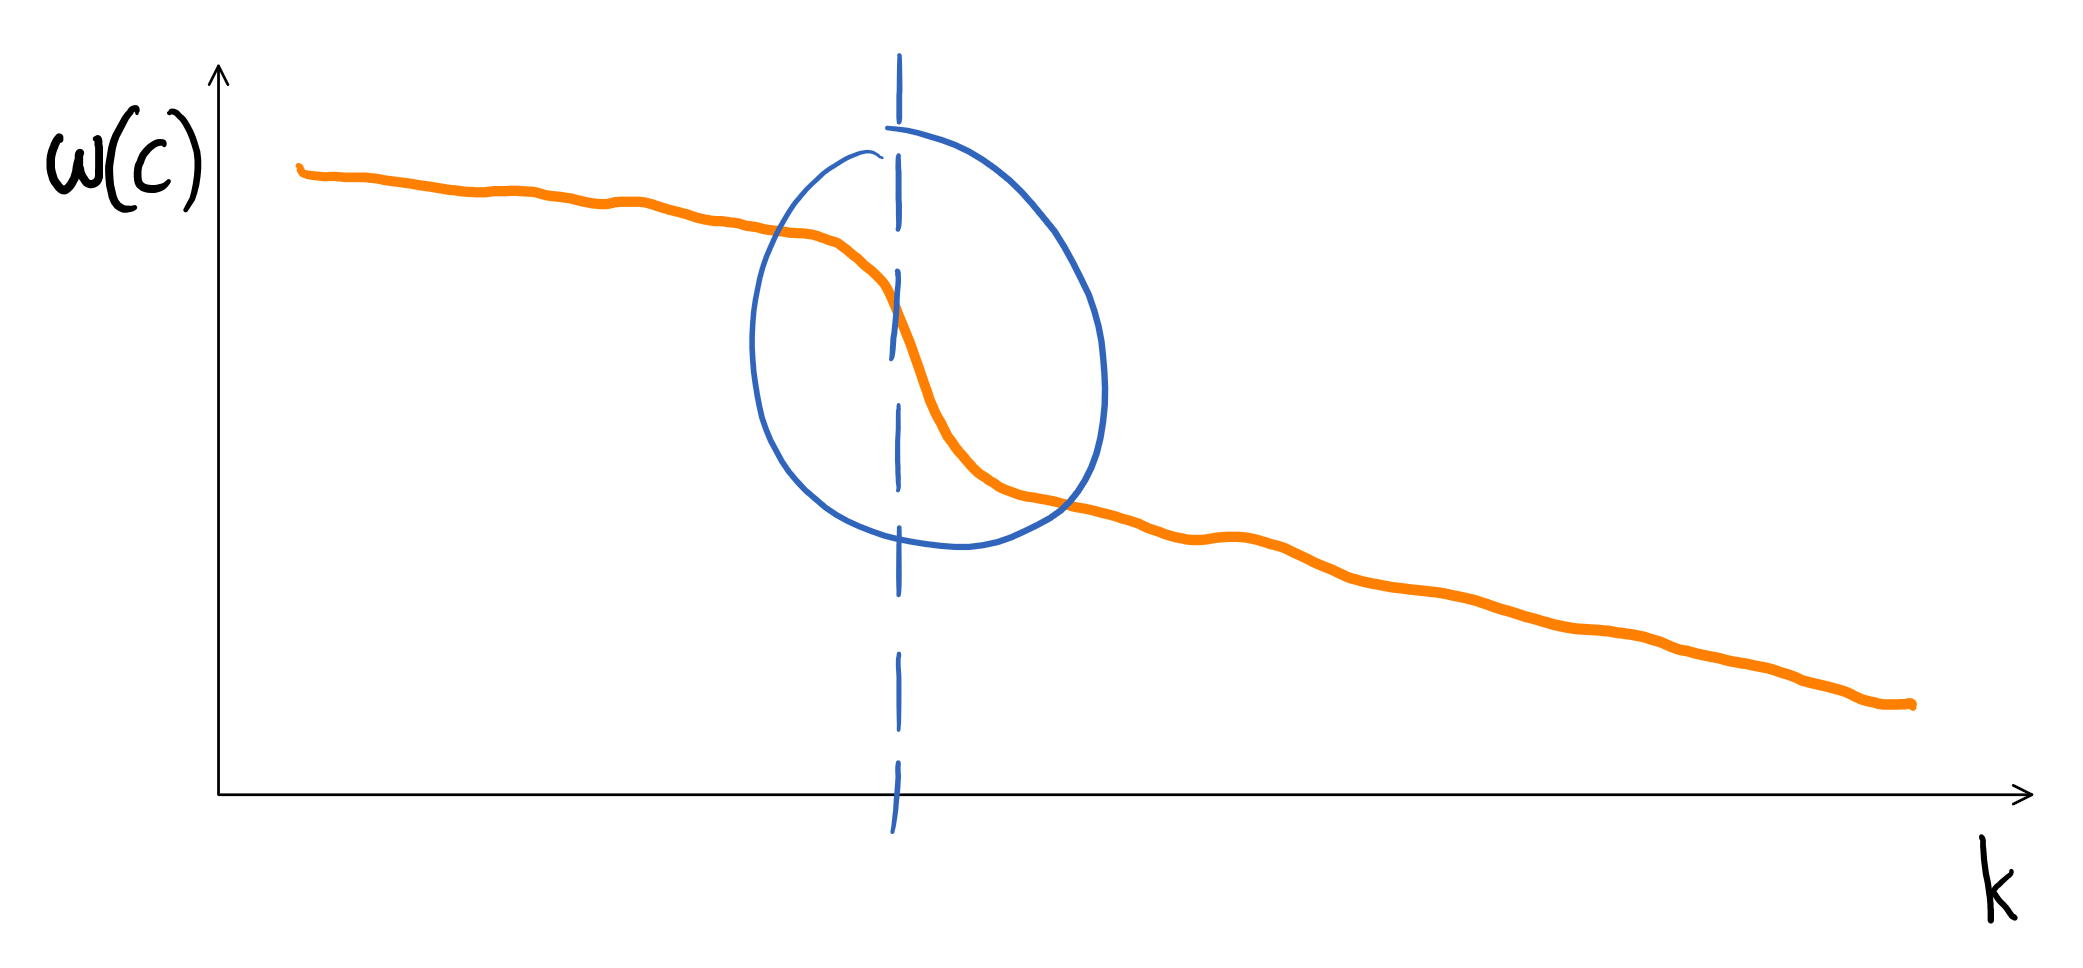
\includegraphics[width=0.8\textwidth]{07-rate-of-change}
\end{figure}

\subparagraph{Approach 2:} Let $w'(c)$ be a metric on a uniform distribution of samples. Relate change of $w(c)$ to change of $w'(c)$. Proposed in TEoSL.

\begin{figure}[H]
	\centering
	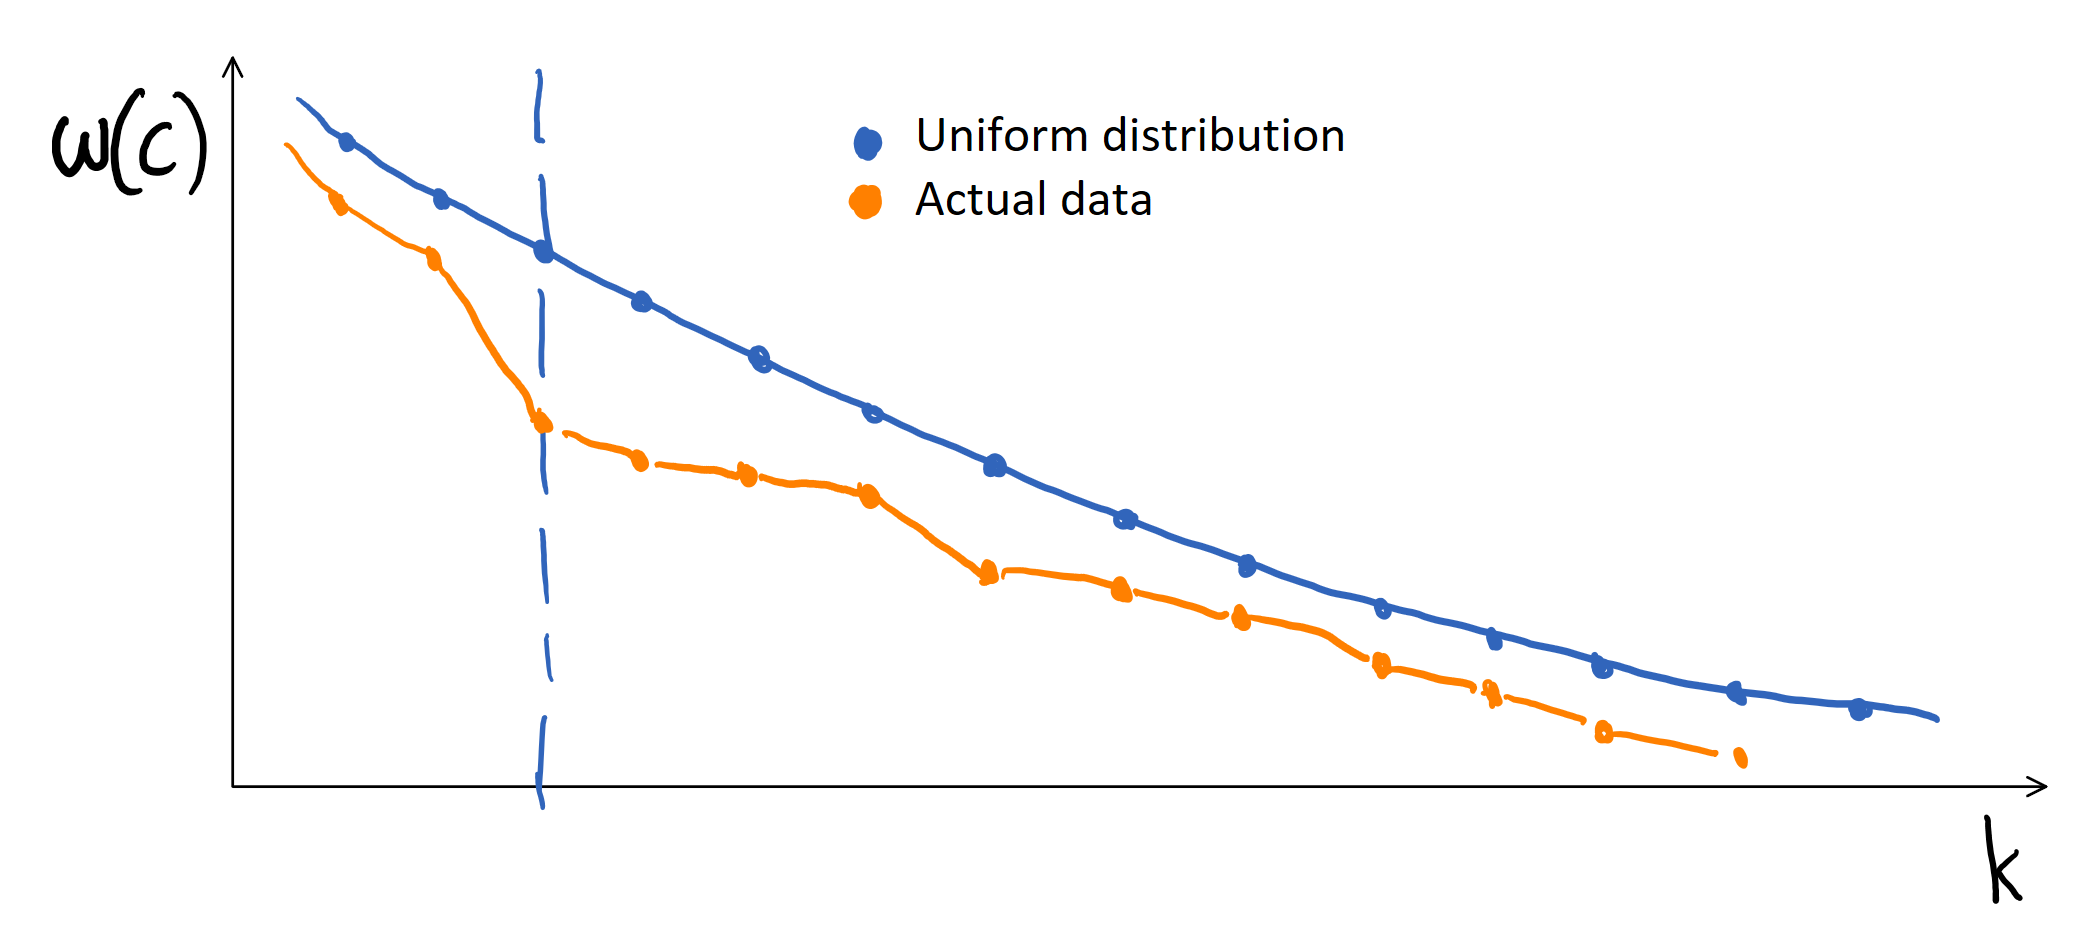
\includegraphics[width=0.8\textwidth]{08-w_c-vs-w_prime_c}
\end{figure}

??? is something missing here ???

We have several options for clustering data. K-means and its variants are straight forward and easy to understand. But if the proper number of clusters is part of the unknowns, it may be a suboptimal choice.
One alternative is mean shift clustering. Here is the number of clusters determined implicitly by the kernel type and size plus the type of bump post process.

Now we will look into a Dirichlet Process to model infinite gaussian mixtures.

\paragraph{The idea for infinite mixture models:}
Instead of fitting a specific distribution to the data (the GMM), we define a meta-distribution from which the actual distribution is drawn.
specifically we can draw a GMM from a dirichlet process\footnote{Because uniform ??? parameters for drawing the GMM}. However this is a top-down perspective, i.e. if we randomly draw a GMM, we will certainly not draw one that fits nicely to our data.
From a bottom up perspective, we need a fitting algorithm that works with the available data points and finds a GMM in such a way, that it could also have been drawn from a distribution of distributions (the dirichlet process).

\paragraph{Chinese restaurant process:}
To illustrate the model behind the fitting algorithm, we usually talk about the ``Chinese restaurant process''.

\begin{figure}[H]
	\centering
	
\includegraphics[width=0.8\textwidth]{todo}
\end{figure}

\paragraph{Extensions to a ``normal'' GMM:}
\begin{enumerate}
	\item If a customer prefers to sit at a new table, this is possible we can add arbitrary many tables
	\item The more people sit on a table  the more attractive it is to the new customers (rich get richer)
\end{enumerate}

The chinese restaurant process (CRP) provides a constructive way of sampling from a dirichlet process.

\paragraph{Gibbs sampling:}
A straight forward clustering algorthm based on the CRP

while(true)

???

Tis is a probailistic algorithm, bcause we sample from the list ..???.

\paragraph{Back to the top-down view:}
Using the CRP, we are effectivly drawing a GMM using a dirichlet process. Implicitly, the mixture weihts $\beta_i$ match a $Beta(\alpha)$ distribution and the normal distributions are drawn from a hyper-distribution, i.e. $\vartheta_i \sim H(\lambda)$

\paragraph{Stick breaking process:}
(Illustration of a $Beta$ distribution)

\begin{figure}[H]
	\centering
	
\includegraphics[width=0.5\textwidth]{todo}
\end{figure}

Qualitatively, this is what the $Beta$ distribution looks like:

\begin{figure}[H]
	\centering
	
\includegraphics[width=0.5\textwidth]{todo}
\end{figure}

The expansion parameter $\alpha$ is a prior that influences the number of clusters that will be created.

\paragraph{Observation 1:}
The larger the expansion parameter $\alpha$ is, the more likely it is to draw a number that is close to $0$ form $Beta(1,\alpha)$

\begin{figure}[H]
	\centering
	
\includegraphics[width=0.5\textwidth]{todo}
\end{figure}

The number that has been drawn form $Beta(1,\alpha)$ is used in the stick breaking process to determine the weight of the i-th mixture component $\beta_i$

\paragraph{Stick breaking process (again):}

\begin{equation*}
	b_i \sim Beta(1,\alpha)
\end{equation*}

\begin{equation*}
	\beta_i = b_i \dot \prod_{i=1}^{i-1}(1-b_i) = b_i (1 - \sum_{i=1}^{i-1} \beta_i)
\end{equation*}

\begin{figure}[H]
	\centering
	
\includegraphics[width=0.5\textwidth]{todo}
\end{figure}
